\documentclass{scrartcl}\usepackage[]{graphicx}\usepackage[]{color}
%% maxwidth is the original width if it is less than linewidth
%% otherwise use linewidth (to make sure the graphics do not exceed the margin)
\makeatletter
\def\maxwidth{ %
  \ifdim\Gin@nat@width>\linewidth
    \linewidth
  \else
    \Gin@nat@width
  \fi
}
\makeatother

\definecolor{fgcolor}{rgb}{0.345, 0.345, 0.345}
\newcommand{\hlnum}[1]{\textcolor[rgb]{0.686,0.059,0.569}{#1}}%
\newcommand{\hlstr}[1]{\textcolor[rgb]{0.192,0.494,0.8}{#1}}%
\newcommand{\hlcom}[1]{\textcolor[rgb]{0.678,0.584,0.686}{\textit{#1}}}%
\newcommand{\hlopt}[1]{\textcolor[rgb]{0,0,0}{#1}}%
\newcommand{\hlstd}[1]{\textcolor[rgb]{0.345,0.345,0.345}{#1}}%
\newcommand{\hlkwa}[1]{\textcolor[rgb]{0.161,0.373,0.58}{\textbf{#1}}}%
\newcommand{\hlkwb}[1]{\textcolor[rgb]{0.69,0.353,0.396}{#1}}%
\newcommand{\hlkwc}[1]{\textcolor[rgb]{0.333,0.667,0.333}{#1}}%
\newcommand{\hlkwd}[1]{\textcolor[rgb]{0.737,0.353,0.396}{\textbf{#1}}}%
\let\hlipl\hlkwb

\usepackage{framed}
\makeatletter
\newenvironment{kframe}{%
 \def\at@end@of@kframe{}%
 \ifinner\ifhmode%
  \def\at@end@of@kframe{\end{minipage}}%
  \begin{minipage}{\columnwidth}%
 \fi\fi%
 \def\FrameCommand##1{\hskip\@totalleftmargin \hskip-\fboxsep
 \colorbox{shadecolor}{##1}\hskip-\fboxsep
     % There is no \\@totalrightmargin, so:
     \hskip-\linewidth \hskip-\@totalleftmargin \hskip\columnwidth}%
 \MakeFramed {\advance\hsize-\width
   \@totalleftmargin\z@ \linewidth\hsize
   \@setminipage}}%
 {\par\unskip\endMakeFramed%
 \at@end@of@kframe}
\makeatother

\definecolor{shadecolor}{rgb}{.97, .97, .97}
\definecolor{messagecolor}{rgb}{0, 0, 0}
\definecolor{warningcolor}{rgb}{1, 0, 1}
\definecolor{errorcolor}{rgb}{1, 0, 0}
\newenvironment{knitrout}{}{} % an empty environment to be redefined in TeX

\usepackage{alltt}
\author{Konrad Medicus, Fabian Oberreiter,Tobias Hilgart}

\usepackage{babel,amsmath, amsthm}
\usepackage{hyperref}
\hypersetup{
    colorlinks=true, %set true if you want colored links
    linktoc=all,     %set to all if you want both sections and subsections linked
    linkcolor=blue,  %choose some color if you want links to stand out
}
\IfFileExists{upquote.sty}{\usepackage{upquote}}{}
\begin{document}

\title{QAD-Package}

\maketitle

\tableofcontents

\section{Introduction}

The \textit{"Quantification of Asymmetric Dependence"} package introduces a copula-based dependency measure capable of detecting and depicting asymmetry.

Dependency measures such as the various correlations are not applicable to measure asymmetric dependence. Using copulae, which describe the joint distribution of a random vector $(X,Y)$ one can 'measure' the distance of a given copula to independence (dependency measure $\zeta_1$, Trutschnig 2011, note) and fullfill all requirements for an asymmetric dependency measure, such as invariant under scale changes, 1 iff $Y$ is a function of $X$, 0 iff independent etc.

However, when one works with samples -- observations $(x_1,y_1),\dots,(x_n,y_n)$ -- the true distribution they are drawn from is generally unknown, and so is the copula then.

Thus there is a need to find a 'good estimate' for said copula in the sense, that it gives a good estimate of the dependency measure.

However, in said measure, the 'known' approximation called \textit{empirical copula} (corresponds to empirical distribution) does not provide a good estimate.

This package introduces a 'smooth aggregation' of the empirical copula, called \textit{empirical checkerboard copula}, that does provide a good estimates and enables the user to estimate the (asymmetric) dependence from a sample by using it.

\section{qad}

The qad -- function does exactly that: From a given data.frame containing a bivariate sample -- on column per variable-- it calculates the empirical checkerboard copula and computes the dependency measure, thus quantifying the asymmetric dependence (qad) of two random variables $X$ and $Y$.

\subsection{Example I}


\begin{knitrout}
\definecolor{shadecolor}{rgb}{0.969, 0.969, 0.969}\color{fgcolor}\begin{kframe}
\begin{alltt}
\hlstd{n} \hlkwb{=} \hlnum{200}
\hlstd{x} \hlkwb{=} \hlkwd{runif}\hlstd{(n,}\hlopt{-}\hlnum{2}\hlstd{,}\hlnum{4}\hlstd{)}
\hlstd{y} \hlkwb{=} \hlkwd{sin}\hlstd{(x}\hlopt{^}\hlnum{2}\hlstd{)}
\hlstd{df} \hlkwb{=} \hlkwd{data.frame}\hlstd{(x,y)}
\hlstd{model} \hlkwb{=} \hlkwd{qad}\hlstd{(df,} \hlkwc{print} \hlstd{=} \hlnum{FALSE}\hlstd{,} \hlkwc{permutation} \hlstd{=} \hlnum{TRUE}\hlstd{)}
\hlstd{model}\hlopt{$}\hlstd{results}
\end{alltt}
\begin{verbatim}
##                        coef p.values
## 1        q(x1,x2) 0.6610848        0
## 2        q(x2,x1) 0.3781406        0
## 3 mean.dependence 0.5196127        0
## 4 asymmetry       0.2829442        0
\end{verbatim}
\end{kframe}
\end{knitrout}

A permutated p-test can be performed to test for independence. The summary function can also be called on qad-objects. With pairwise.qad, one can calculate the qad for each pair of columns in a given data.frame, and heatmap.qad visualizes the results.

\subsection{Example II}
\begin{knitrout}
\definecolor{shadecolor}{rgb}{0.969, 0.969, 0.969}\color{fgcolor}\begin{kframe}
\begin{alltt}
  \hlkwd{load}\hlstd{(}\hlkwd{url}\hlstd{(}\hlstr{"http://www.trutschnig.net/RTR.RData"}\hlstd{))}
  \hlstd{df} \hlkwb{=} \hlstd{RTR[}\hlkwd{sample}\hlstd{(}\hlkwd{nrow}\hlstd{(RTR),}\hlnum{1000}\hlstd{),}
           \hlkwd{c}\hlstd{(}\hlstr{'long'}\hlstd{,}\hlstr{'lat'}\hlstd{,}\hlstr{'rtr_speed_dl'}\hlstd{,}\hlstr{'rtr_speed_ul'}\hlstd{)]}
  \hlstd{model} \hlkwb{=} \hlkwd{pairwise.qad}\hlstd{(df)}
\end{alltt}
\begin{verbatim}
## [1] "Process..."
## [1] "Process: 1 / 4"
## [1] "Process: 2 / 4"
## [1] "Process: 3 / 4"
\end{verbatim}
\begin{alltt}
  \hlkwd{heatmap.qad}\hlstd{(model)}
\end{alltt}
\end{kframe}
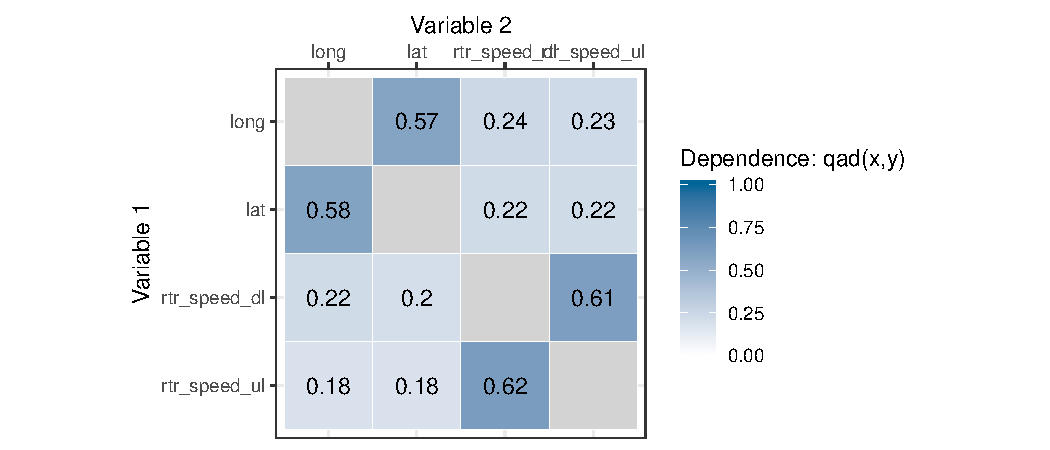
\includegraphics[width=\maxwidth]{figure/unnamed-chunk-3-1} 

\end{knitrout}

\section{cci}

Gives a confidence intervall, depending on the sample size, for the qad measure of two independent random variables. Thus, it can be used to test for independence.

\begin{knitrout}
\definecolor{shadecolor}{rgb}{0.969, 0.969, 0.969}\color{fgcolor}\begin{kframe}
\begin{alltt}
\hlstd{c} \hlkwb{=} \hlkwd{cci}\hlstd{(n,} \hlkwc{alternative} \hlstd{=} \hlstr{"one.sided"}\hlstd{)}

\hlstd{x} \hlkwb{=} \hlkwd{runif}\hlstd{(n,}\hlopt{-}\hlnum{2}\hlstd{,}\hlnum{4}\hlstd{)}
\hlstd{y} \hlkwb{=} \hlkwd{sin}\hlstd{(x}\hlopt{^}\hlnum{2}\hlstd{)}
\hlstd{df} \hlkwb{=} \hlkwd{data.frame}\hlstd{(x,y)}
\hlstd{model} \hlkwb{=} \hlkwd{qad}\hlstd{(df,}\hlkwc{print}\hlstd{=}\hlnum{FALSE}\hlstd{)}

\hlkwa{if}\hlstd{(}\hlkwd{coef}\hlstd{(model,} \hlkwc{select} \hlstd{=} \hlstr{'q(x1,x2)'}\hlstd{)} \hlopt \hlstd{c)\{}
 \hlkwd{print}\hlstd{(}\hlstr{'Accept H0'}\hlstd{)}
\hlstd{\}}\hlkwa{else}\hlstd{\{}
 \hlkwd{print}\hlstd{(}\hlstr{'Reject H0'}\hlstd{)}
\hlstd{\}}
\end{alltt}
\begin{verbatim}
## [1] "Reject H0"
\end{verbatim}
\end{kframe}
\end{knitrout}

\section{the rest \\ plot/predict/emp\_ c\_ copula/plot\_ density}

If one desires to calculate just the empirical copula (smoothing=FALSE) or the checkerboard aggregation (smoothing=TRUE), one can do so by plugging the data.frame(x,y) into the emp\_ c\_ copula() -- function. The resulting mass/density matrix can be plotted via plot\_ density.

Alternatively, calling the plot -- function on a qad-object directly plots it's mass matrix (from the checkerboard aggregation), one can also add the sample points and retransform from the copula into the original data setting.

Using the conditional probabilities, with the predict command on a qad-object, one gets the probabilities to land in certain intervals, given either certain $x$ or $y$ values (after specifying which are given). One can manually set the number of intervals, into which the range of the other RV is splitted.

\subsection{Example I}
\begin{knitrout}
\definecolor{shadecolor}{rgb}{0.969, 0.969, 0.969}\color{fgcolor}\begin{kframe}
\begin{alltt}
\hlkwd{set.seed}\hlstd{(}\hlnum{2019}\hlstd{)}
\hlstd{x} \hlkwb{=} \hlkwd{rnorm}\hlstd{(}\hlnum{50}\hlstd{,}\hlnum{1}\hlstd{,}\hlnum{2}\hlstd{)}
\hlstd{y} \hlkwb{=} \hlstd{x}\hlopt{^}\hlnum{2} \hlopt{+} \hlkwd{rnorm}\hlstd{(}\hlnum{50}\hlstd{,}\hlnum{0}\hlstd{,}\hlnum{1}\hlstd{)}
\hlstd{df} \hlkwb{=} \hlkwd{data.frame}\hlstd{(x,y)}

\hlstd{ECC} \hlkwb{=} \hlkwd{emp_c_copula}\hlstd{(df,} \hlkwc{resolution} \hlstd{=} \hlnum{7}\hlstd{)}
\hlkwd{plot_density}\hlstd{(ECC,}\hlkwc{density}\hlstd{=}\hlnum{FALSE}\hlstd{)}
\end{alltt}
\end{kframe}
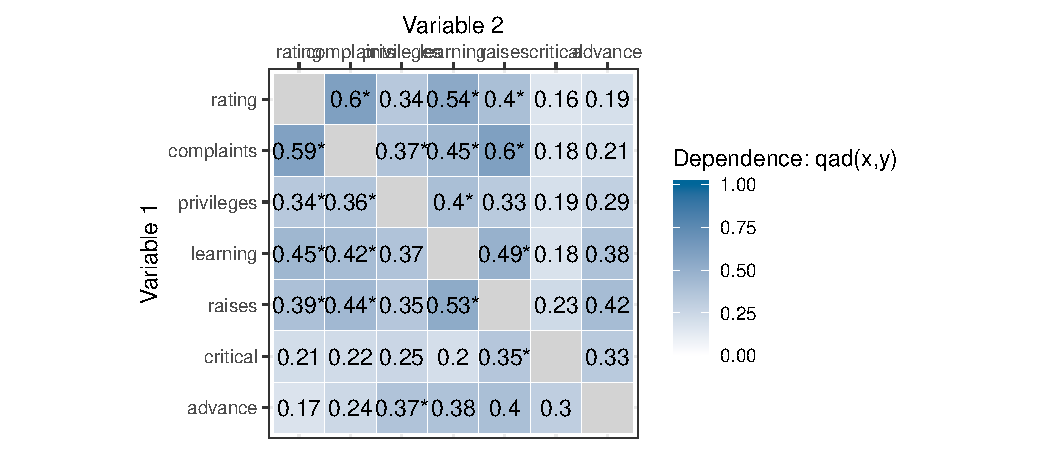
\includegraphics[width=\maxwidth]{figure/unnamed-chunk-5-1} 

\end{knitrout}

\begin{knitrout}
\definecolor{shadecolor}{rgb}{0.969, 0.969, 0.969}\color{fgcolor}\begin{kframe}
\begin{alltt}
\hlstd{model} \hlkwb{=} \hlkwd{qad}\hlstd{(df,}\hlkwc{print}\hlstd{=}\hlnum{FALSE}\hlstd{)}
\hlkwd{plot}\hlstd{(model,} \hlkwc{copula} \hlstd{=} \hlnum{TRUE}\hlstd{)}
\end{alltt}
\end{kframe}
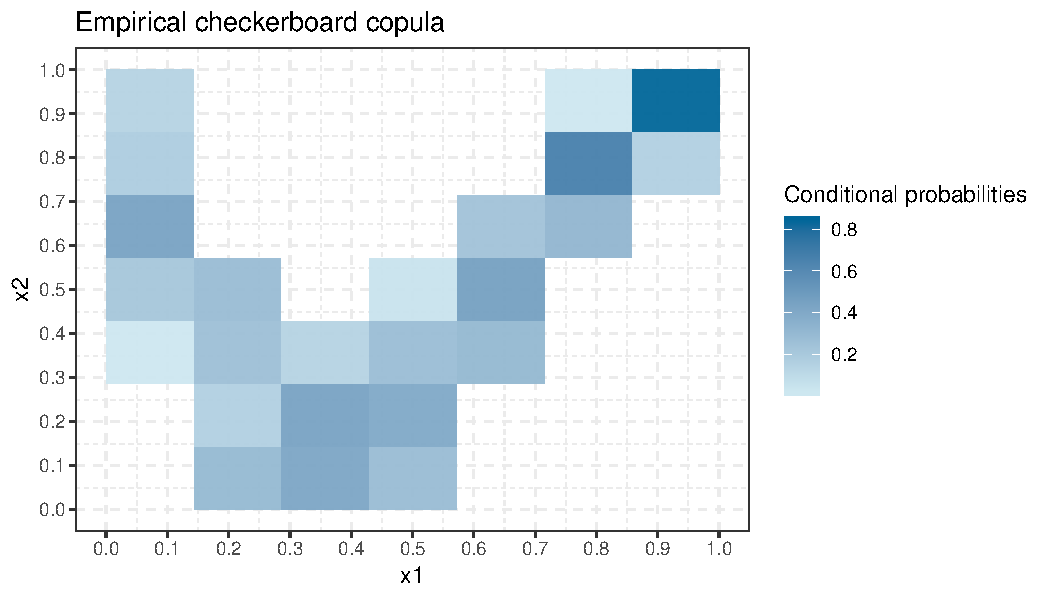
\includegraphics[width=\maxwidth]{figure/unnamed-chunk-6-1} 

\end{knitrout}


\subsection{Example II}
\begin{knitrout}
\definecolor{shadecolor}{rgb}{0.969, 0.969, 0.969}\color{fgcolor}\begin{kframe}
\begin{alltt}
\hlkwd{predict}\hlstd{(model,} \hlkwc{values} \hlstd{=} \hlkwd{c}\hlstd{(}\hlopt{-}\hlnum{1}\hlstd{,}\hlnum{0}\hlstd{,}\hlnum{1}\hlstd{,}\hlnum{2}\hlstd{,}\hlnum{3}\hlstd{),} \hlkwc{conditioned} \hlstd{=} \hlstr{"x1"}\hlstd{,}
        \hlkwc{nr_intervals} \hlstd{=} \hlnum{5}\hlstd{)}
\end{alltt}
\begin{verbatim}
##    (-0.73,0.5] (0.5,1.87] (1.87,4.9] (4.9,7.27] (7.27,39.82]
## -1       0.364  0.3040000  0.3320000      0.000        0.000
## 0        0.596  0.3760000  0.0280000      0.000        0.000
## 1        0.440  0.4594286  0.1005714      0.000        0.000
## 2        0.000  0.2445714  0.5634286      0.192        0.000
## 3        0.000  0.0000000  0.0000000      0.096        0.904
\end{verbatim}
\end{kframe}
\end{knitrout}


\end{document}
